% Template for Cogsci submission with R Markdown

% Stuff changed from original Markdown PLOS Template
\documentclass[10pt, letterpaper]{article}

\usepackage{cogsci}
\usepackage{pslatex}
\usepackage{float}
\usepackage{caption}

% amsmath package, useful for mathematical formulas
\usepackage{amsmath}

% amssymb package, useful for mathematical symbols
\usepackage{amssymb}

% hyperref package, useful for hyperlinks
\usepackage{hyperref}

% graphicx package, useful for including eps and pdf graphics
% include graphics with the command \includegraphics
\usepackage{graphicx}

% Sweave(-like)
\usepackage{fancyvrb}
\DefineVerbatimEnvironment{Sinput}{Verbatim}{fontshape=sl}
\DefineVerbatimEnvironment{Soutput}{Verbatim}{}
\DefineVerbatimEnvironment{Scode}{Verbatim}{fontshape=sl}
\newenvironment{Schunk}{}{}
\DefineVerbatimEnvironment{Code}{Verbatim}{}
\DefineVerbatimEnvironment{CodeInput}{Verbatim}{fontshape=sl}
\DefineVerbatimEnvironment{CodeOutput}{Verbatim}{}
\newenvironment{CodeChunk}{}{}

% cite package, to clean up citations in the main text. Do not remove.
\usepackage{apacite}

% KM added 1/4/18 to allow control of blind submission
\cogscifinalcopy

\usepackage{color}

% Use doublespacing - comment out for single spacing
%\usepackage{setspace}
%\doublespacing


% % Text layout
% \topmargin 0.0cm
% \oddsidemargin 0.5cm
% \evensidemargin 0.5cm
% \textwidth 16cm
% \textheight 21cm

\title{Title TBD}


\author{Kennedy Casey \\
        University of Chicago \\
        \texttt{kbcasey@uchicago.edu}
\And \textbf{Elizabeth Mickiewicz} \\
             University of Chicago \\
             \texttt{lizmick9@uchicago.edu}
\And \textbf{Kimberly Shorter} \\
             University of Chicago \\
             \texttt{klshorter@uchicago.edu}
\And \textbf{Anapaula Silva Mandujano} \\
             University of Chicago \\
             \texttt{anapaula@uchicago.edu}            
\AND \textbf{Mara Duquette} \\
             University of Chicago \\
             \texttt{duquettemara@uchicago.edu}
\And \textbf{Mary Elliott} \\
             University of Texas at Dallas \\
             \texttt{maryle18@gmail.com}
\And \textbf{Elika Bergelson} \\
             Duke University \\
             \texttt{elika.bergelson@duke.edu}
\And \textbf{Marisa Casillas} \\
             University of Chicago \\
             \texttt{mcasillas@uchicago.edu}}


\begin{document}

\maketitle

\begin{abstract}


\textbf{Keywords:}

\end{abstract}

\hypertarget{introduction}{%
\section{Introduction}\label{introduction}}

The artifacts of everyday life reflect our routines, aspirations,
relationships, and much more. In particular, the objects that we
regularly pick up and handle---a coffee cup, a laptop, a baby
bottle---offer a window into the physical, social, and cultural contexts
that shape our understanding of the world. In this paper, we take a
glimpse into everyday life at its beginnings by exploring home object
handling from early infancy until age four. We discuss the implications
of the findings for models of word learning.

\hypertarget{object-handling-and-word-learning}{%
\subsection{Object handling and word
learning}\label{object-handling-and-word-learning}}

For young learners, objects and their associated activities form a
critical source of input for social learning, including the ways in
which children are exposed to language about those objects (see
(\textbf{herzberg2021exuberant?}) for an overview of object play and
motor learning). More generally, hands (and what they are handling) can
be reliable indicators of what someone is doing and talking about during
object play, facilitating children's ability to map word forms onto
their meanings in and across real-time interaction (e.g.,
\textbf{yu2013joint?}; \textbf{yurovsky2013statistical?}). Present,
attended-to objects also influence the babble of children with stable
consonants (\textbf{laing2020babble?}). And caregivers' tendency to use
nouns referring to objects in the here-and-now positively predicts their
children's early word comprehension (\textbf{bergelson2017nature?}).

How frequently do children encounter held objects? Hands---others' and
their own---are in good supply in young children's view of the world,
especially after early infancy (\textbf{fausey2016faces?};
\textbf{jayaraman2017faces?}; but see \textbf{long2020detecting?}),
topping out at visible presence \textasciitilde30\% of the time. Infants
own object handling is also relatively frequent: Herzberg and colleagues
(\textbf{herzberg2021exuberant?}) find that infants handle objects
\textasciitilde60\% of the time during at-home play, Yu and colleagues
(\textbf{yu2013joint?}) find \textasciitilde70\% when including joint
handling with adults in US in-lab object play, and
(\textbf{casillasURdaylong?}) find \textasciitilde15 and
\textasciitilde17\% object handling in day-long photo streams in a
Papuan and a Mayan community, respectively. Note, however, that the
likelihood of talk about objects that are being handled in the here and
now---a flagship feature of contingent caregiver talk
(\textbf{mcgillion2017randomised?})---fluctuates across high and low
activity periods of interaction (\textbf{bergelson2019day?}).

In sum, prior work points to the immense potential of children's
object-centric interactions for their word learning, but little work has
yet begun to examine the types of objects children typically interact
with at home and how object handling changes across age and varies
across cultural contexts (\textbf{herzberg2021exuberant?}).

\hypertarget{object-handling-across-age-and-culture}{%
\subsection{Object handling across age and
culture}\label{object-handling-across-age-and-culture}}

This object-centered input changes enormously across the first few years
due to both maturational constraints and culture-specific caregiving
practices. In early infancy, children have little ability to hold things
or to control their posture, primarily experiencing objects through what
others bring near to them (faces may make up a much greater proportion
of their social input at this point; fauseyREF). However, later gains in
manual dexterity and gross motor skill (e.g., sitting, crawling,
walking) increasingly widen their ability to seek, reach, and grab a
diversity of objects in their environment and give them greater control
over what they handle, how, and for how long (REFS).

Separately, early access to objects is shaped by culture-specific
practices for carrying children, keeping them safe and warm, and
scaffolding the development of locally valued capacities (e.g., word
learning in many US families, walking in Kenyan Kipsigis families,
(\textbf{super1976environmental?})), which may slightly alter the course
of motor development (see (\textbf{adolph2010motor?}) for an overview).

The array of objects available to children will also vary
crossculturally, including: (a) objects spread via globalization (e.g.,
plastic bags), (b) objects that have a basic functional role that is
similar across contexts (e.g., spoon-like things for eating), and (c)
objects are specific to people and places (e.g., the gourd and bombilla
for drinking mate in much of South America, stemming from Indigenous
Guaraní and Tupí tradition). Take, for example, middle-class US family
homes, which have been noted for their large quantities of possessions
(``clutter''), much of which is designed specifically for children
(e.g., toys and books (\textbf{arnold2017life?})). We might infer based
on this distribution of objects that much of what children do and talk
about at home is tailored to what particularly interests them and thus
children's worlds, in this sense, look very different from adults'.
Recent work by Herzberg and colleagues (\textbf{herzberg2021exuberant?})
underscores this point with infancy data; 13--23-month-olds spent nearly
70\% of their time in object play with toys or a mix of toys and
non-toys, with \textasciitilde100\% of infants playing with children's
books and stuffed animals and a total of 32 toy types appearing in
\(\ge\) 25\% of infants' play. Non-toy play was also common, but still
appeared to predominantly include infant-specific objects (e.g., sippy
cups, baby spoons, high chairs, pacifiers). We would expect many of
these items to be rare in other parts of the world, with much greater
overlap between objects for infants and objects for adults (e.g.,
(\textbf{karasik2018not?})).

\hypertarget{methods}{%
\section{Methods}\label{methods}}

\hypertarget{corpus}{%
\subsection{Corpus}\label{corpus}}

Daylong photo streams consist of images captured every 15 (Rossel) to 30
(Tseltal) seconds over the course of 8 (Rossel) to 9 (Tseltal) hours at
home. Children wore a recording vest equipped with a camera (Narrative
Clip 1) and miniature fisheye lens (Photojojo Super Fisheye) that
provided a 180\(\text{\textdegree}\) frontal view of the child's
environment (Narrative Clip 1). For younger infants who were not yet
walking, the camera was instead worn by the primary caregiver. Here, we
analyze the subset of photos known to contain child object handling
based on prior work with the same data sets
(\textbf{casillas2021crosscultural?}).

These data include XX children (Rossel: XX, Tseltal: XX) ranging in age
from X to XX months (\emph{M}\textsubscript{\emph{Rossel}} = XX.X,
\emph{M}\textsubscript{\emph{Tseltal}} = XX.X). For each child, a range
of X-XXX photos were annotated (\emph{M}\textsubscript{\emph{Rossel}} =
XX.X, \emph{M}\textsubscript{\emph{Tseltal}} = XX.X).

\hypertarget{manual-annotation}{%
\subsection{Manual annotation}\label{manual-annotation}}

We annotated photos with IMCO (version 2; GitHub link removed for blind
review), an open-source program adapted for efficient coding of photo
streams. Annotators provided labels for the handled object(s) present in
each photo and selected among 12 predefined object types to describe
each object: food, clothing, toys, books, electronic devices, plants,
animals, tools (for work/cleaning), tools (for mealtime), other large or
immovable objects, other synthetic objects, and other natural objects.
For analyses reported below, we collapsed across this set of object
types to yield 6 categories of common objects: food, tools, toys,
immovable objects, miscellaneous natural objects, and miscellaneous
synthetic objects (see Table \ref{tab:top-objects} for example objects
from each category),

\hypertarget{reliability}{%
\subsection{Reliability}\label{reliability}}

XX\% of photo streams were double coded. Reliability annotations were
equally spread across sites and ages. At the category level, annotators
agreed on XX.X\% of decisions (Rossel: XX.X\%, Tseltal: XX.X\%). At the
object label level, annotators agreed on XX.X\% of decisions (Rossel:
XX.X\%). Additionally, to avoid unnecessary data loss, all excluded
photos were checked by a second annotator and re-included for analysis
if objects were identifiable.

\begin{table}[!ht]
\centering
\scalebox{0.8}{
\begin{tabular}{lll}
  \hline
Object Category & Rossel & Tseltal \\ 
  \hline
Synthetic & rope, shirt, plastic bottle & shirt, chair, pants \\ 
  Food & coconut, betelnut, tuber & guava, tortilla, apple \\ 
  Tool & knife, bowl, spoon & bowl, cup, bottle \\ 
  Toy & ball, book, plastic toy & book, toy truck, baby doll \\ 
  Natural & stick, rock, leaf & stick, leaf, tree \\ 
  Immovable & veranda, ladder, railing & door, fence, table \\ 
   \hline
\end{tabular}
}
\caption{Objects handled by the most children across categories and sites.} 
\label{tab:top-objects}
\end{table}

\hypertarget{results}{%
\section{Results}\label{results}}

\hypertarget{overall-frequency-statistics}{%
\subsection{Overall frequency
statistics}\label{overall-frequency-statistics}}

Children handled an average of 21.16 unique objects per day (median =
20, \emph{SD} = 15.2, range = 1--59), with no significant differences
across sites (\emph{M}\textsubscript{\emph{Rossel}} = 18.93,
\emph{M}\textsubscript{\emph{Tseltal}} = 23.24, \emph{W} = 350, \emph{p}
= 0.501). Only 20.83\% of objects were present in both communities, but
several shared objects were among the most frequently handled by
children in both sites. In fact, among the top 25 most common objects,
11 were shared across sites.

The frequency of object categories was similarly divided across sites
(Figure 1A). The top objects for each category are shown in Table 1.
Children primarily handled miscellaneous synthetic objects (e.g., rope,
guitar, shirt, etc.; \emph{M}\textsubscript{\emph{Rossel}} = 32.01\% of
handling, \emph{M}\textsubscript{\emph{Tseltal}} = 37.5\%) and food
(\emph{M}\textsubscript{\emph{Rossel}} = 28.58\%,
\emph{M}\textsubscript{\emph{Tseltal}} = 36.21\%). For 45 of 56
children, the top category was either synthetic objects or food.
Two-tailed Wilcoxon tests revealed only one significant category-level
difference between sites: children's handling of large or immovable
objects (e.g., veranda, ladder, railing, etc.), where Rossel children
handled these objects more frequently than Tseltal children
(\emph{M}\textsubscript{\emph{Rossel}} = 7.73\%,
\emph{M}\textsubscript{\emph{Tseltal}} = 3.31\%, adjusted \emph{p} =
0.038, \emph{p}s for all other categories \textgreater{} 0.05), but
these objects were still the least frequently handled in both sites.

During any given hour, children handled 5.26 objects from 2.79 different
categories, on average (median = 4.5 objects, \emph{SD} = 3.92, range =
1--18). A linear mixed-effects model with fixed effects of site, each of
6 object categories, and their interaction showed a significant main
effect of the synthetic object category (\(\beta\) = 0.52, \emph{SE} =
0.2, \emph{t} = 2.59, \emph{p} = 0.01) as well as an interaction between
site and the synthetic object category (\(\beta\) = 1.11, \emph{SE} =
0.29, \emph{t} = 3.88, \emph{p} = \textless{} 0.001) such that children
handled more unique synthetic objects per hour than any other object
category, and this effect was stronger for Tseltal children than for
Rossel children (\emph{p}s \textgreater{} 0.05 for all other main
effects and interaction terms; Figure 1B).

\begin{CodeChunk}
\begin{figure}[!ht]

{\centering 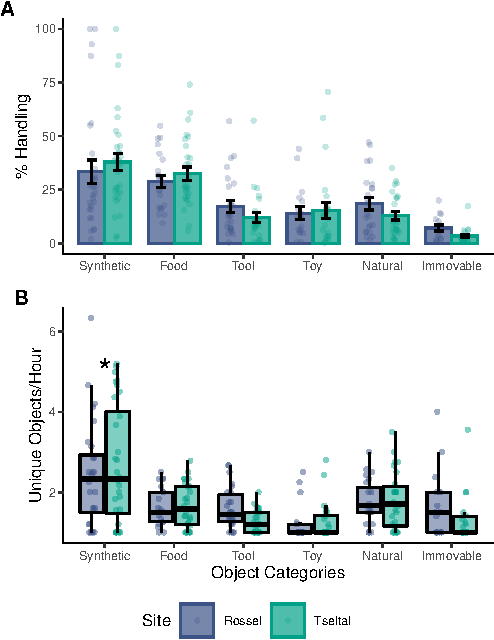
\includegraphics{figs/overall-stats-fig-1} 

}

\caption[(A) Overall frequency of handling by object category]{(A) Overall frequency of handling by object category. Points reflect percentages for individual children. (B) Count of unique objects handled per hour by object category. Points reflect means for individual children across all hours of recording.}\label{fig:overall-stats-fig}
\end{figure}
\end{CodeChunk}

\hypertarget{time-of-day-effects}{%
\subsection{Time of day effects}\label{time-of-day-effects}}

Children's overall rate of object handling was largely consistent across
the day. The number of unique handled objects per hour was not linearly
related to time of day (\(\beta\) = -0.02, \emph{SE} = 0.11, \emph{t} =
-0.16, \emph{p} = 0.874), and there was no two-way interaction between
time of day and site (\(\beta\) = 0.01, \emph{SE} = 0.14, \emph{t} =
0.1, \emph{p} = 0.923).

However, we did find differences in children's rates of holding for
specific object categories across the day. We ran individual linear
mixed-effects models, which included fixed effects of site, hour of the
day, and their interaction, for each of 6 categories. Synthetic objects
were marginally more common during the afternoon hours (\(\beta\) =
0.02, \emph{SE} = 0.01, \emph{t} = 1.71, \emph{p} = 0.09), and food
items were handled with significantly greater frequency during the
morning hours (\(\beta\) = -0.03, \emph{SE} = 0.01, \emph{t} = -2.76,
\emph{p} = 0.006; Figure 2). No other main effects or two-way
interactions reached statistical significance (all \emph{p}s
\textgreater{} 0.05).

\begin{CodeChunk}
\begin{figure}[!ht]

{\centering 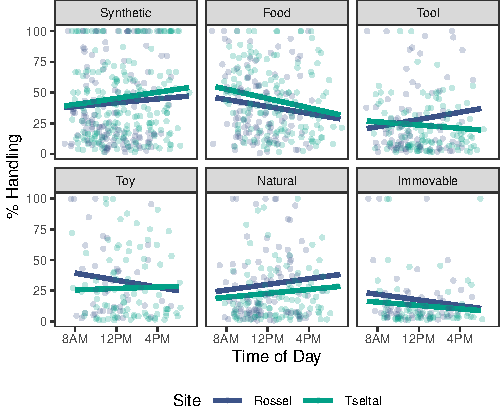
\includegraphics{figs/tod-effects-fig-1} 

}

\caption[Frequency of handling by object category across different times of day]{Frequency of handling by object category across different times of day. Individual points show raw percentages for each child, and lines reflect model-predicted percentages.}\label{fig:tod-effects-fig}
\end{figure}
\end{CodeChunk}

\hypertarget{age-effects}{%
\subsection{Age effects}\label{age-effects}}

Children's overall rate of object handling increased marginally with age
(Figure 3A). That is, older children handled more unique objects per
hour (\(\beta\) = 0.07, \emph{SE} = 0.03, \emph{t} = 1.99, \emph{p} =
0.05). Additionally, with increasing age, children handled more objects
from different categories per hour (\(\beta\) = 0.03, \emph{SE} = 0.01,
\emph{t} = 2.6, \emph{p} = 0.011). These effects were consistent across
sites; we found no main effects of site or interactions between site and
age (all \emph{p}s \textgreater{} 0.05).

\begin{CodeChunk}
\begin{figure}[!ht]

{\centering 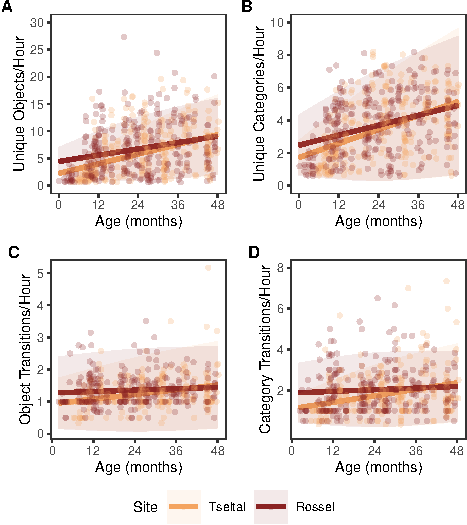
\includegraphics{figs/age-effects-fig-1} 

}

\caption[(A) Unique objects and (B) object categories handled per hour as a function of age]{(A) Unique objects and (B) object categories handled per hour as a function of age. Points reflect raw hourly counts for each child, and lines reflect model predictions with shaded standard error regions.}\label{fig:age-effects-fig}
\end{figure}
\end{CodeChunk}

\hypertarget{discussion}{%
\section{Discussion}\label{discussion}}

\hypertarget{references}{%
\section{References}\label{references}}

\setlength{\parindent}{-0.1in} 
\setlength{\leftskip}{0.125in}

\noindent

\bibliographystyle{apacite}


\end{document}
